% -------------------------------------------------------------
%  Fate’s Edge – Printable Character Sheet (LaTeX)
%  -------------------------------------------------------------
%  Compile with:  pdflatex sheet.tex   (or lualatex/xelatex)
%  -------------------------------------------------------------
\documentclass[paper=a4,landscape,12pt]{article}
\usepackage[margin=1.5cm]{geometry}
\usepackage{fontspec}               % for nice fonts (LuaLaTeX/XeLaTeX)
\usepackage{tikz}
\usepackage{array}
\usepackage{tabularx}
\usepackage{multicol}
\usepackage{pifont}                % for check‑boxes
\usepackage{enumitem}
\usepackage{calc}
\usepackage{titlesec}
\usepackage{booktabs}
\usepackage{setspace}
\usepackage{xcolor}

% -------------------------------------------------------------
%  Simple symbols
\newcommand{\cmark}{\ding{51}}   % checked box
\newcommand{\xmark}{\ding{55}}   % empty box
\newcommand{\blankbox}{\square} % empty square (for hand‑fill)

% -------------------------------------------------------------
%  Colours for quick visual cues (feel free to edit)
\definecolor{dominant}{RGB}{  0,150,  0}   % green
\definecolor{controlled}{RGB}{255,165,  0} % orange
\definecolor{desperate}{RGB}{200,  0,  0}   % red
\definecolor{boon}{RGB}{255,215,  0}       % gold
\definecolor{sb}{RGB}{ 70,130,180}       % steel‑blue

% -------------------------------------------------------------
%  Some column types
\newcolumntype{L}[1]{>{\raggedright\arraybackslash}p{#1}}
\newcolumntype{C}[1]{>{\centering\arraybackslash}p{#1}}
\newcolumntype{R}[1]{>{\raggedleft\arraybackslash}p{#1}}

% -------------------------------------------------------------
%  Title formatting (no numbers, small vertical space)
\titleformat{\section}{\large\bfseries}{}{0pt}{}
\titlespacing*{\section}{0pt}{1.0ex plus .2ex}{0.5ex plus .1ex}
\titleformat{\subsection}{\normalsize\bfseries}{}{0pt}{}
\titlespacing*{\subsection}{0pt}{0.8ex plus .2ex}{0.3ex plus .1ex}

% -------------------------------------------------------------
\begin{document}
\pagestyle{empty}   % no page numbers

% =============================================================
% ========================  FRONT PAGE  =======================
% =============================================================
\begin{tikzpicture}[remember picture,overlay]
  % Light gray background grid (only visible in PDF viewer, not on print)
  \foreach \x in {0,1,...,29}
    {\draw[gray!20] (\x,0) -- (\x,20);}
  \foreach \y in {0,1,...,19}
    {\draw[gray!20] (0,\y) -- (30,\y);}
\end{tikzpicture}

\begin{center}
    {\LARGE \textbf{FATE'S EDGE – CHARACTER SHEET}}\\[0.5ex]
    {\large (Print double‑sided, front on the left, back on the reverse)}
\end{center}
\vspace{0.5cm}

% -----------------------------------------------------------------
% 1. Header block (name, concept, portrait, tier, XP)
% -----------------------------------------------------------------
\noindent\begin{tabularx}{\linewidth}{@{}L{3.2cm} X@{}}
\textbf{Character Name:} & \underline{\hspace{10cm}} \\
\textbf{Player:}          & \underline{\hspace{10cm}} \\
\textbf{Concept / Archetype:} & \underline{\hspace{10cm}} \\
\end{tabularx}

\vspace{0.3cm}
\begin{tabularx}{\linewidth}{@{}L{3.2cm} C{4cm} C{4cm} C{4cm}@{}}
\textbf{Tier:}          & \underline{\hspace{2cm}} & \textbf{XP:} & \underline{\hspace{2cm}} \\
\textbf{Reputation:}    & \underline{\hspace{2cm}} &
\textbf{Campaign Clock:} & \underline{\hspace{2cm}} \\
\end{tabularx}

\vspace{0.5cm}
% -----------------------------------------------------------------
% 2. Core Attributes & Health
% -----------------------------------------------------------------
\noindent\begin{tabularx}{\linewidth}{@{}*4{C{3.5cm}}@{}}
% Attribute circles (filled later by hand)
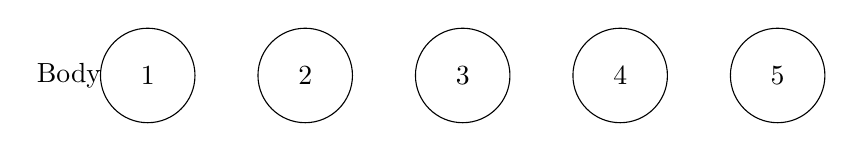
\begin{tikzpicture}
  \foreach \i in {1,...,5}{
    \node[draw,circle,minimum size=1.2cm] (a\i) at (2*\i,0) {};
    \node at (2*\i,0) {$\i$};
  }
  \node at (1,0) {Body};
\end{tikzpicture}
&
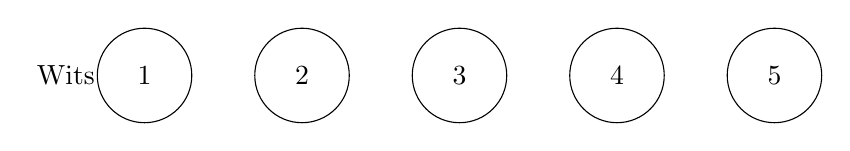
\begin{tikzpicture}
  \foreach \i in {1,...,5}{
    \node[draw,circle,minimum size=1.2cm] (a\i) at (2*\i,0) {};
    \node at (2*\i,0) {$\i$};
  }
  \node at (1,0) {Wits};
\end{tikzpicture}
&
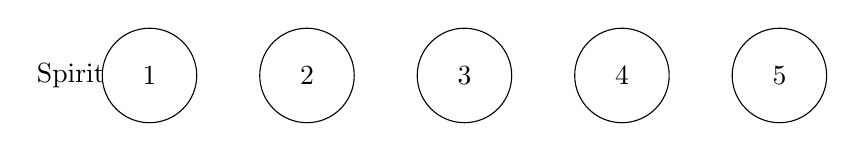
\begin{tikzpicture}
  \foreach \i in {1,...,5}{
    \node[draw,circle,minimum size=1.2cm] (a\i) at (2*\i,0) {};
    \node at (2*\i,0) {$\i$};
  }
  \node at (1,0) {Spirit};
\end{tikzpicture}
&
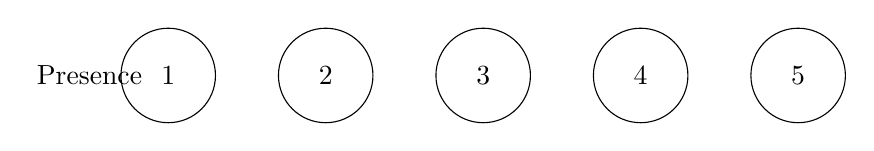
\begin{tikzpicture}
  \foreach \i in {1,...,5}{
    \node[draw,circle,minimum size=1.2cm] (a\i) at (2*\i,0) {};
    \node at (2*\i,0) {$\i$};
  }
  \node at (1,0) {Presence};
\end{tikzpicture}
\\[0.2cm]
\multicolumn{4}{c}{\textbf{Harm / Fatigue Tracker}}\\[0.1cm]
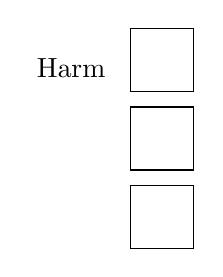
\begin{tikzpicture}
  \foreach \i in {1,...,3}{
    \draw (0,-\i) rectangle (0.8,-\i-0.8);
  }
  \node[left] at (-0.2,-1.5) {Harm};
\end{tikzpicture}
&
\begin{tikzpicture}
  \foreach \i in {1,...,5}{
    \draw (0,-\i) rectangle (0.8,-\i-0.8);
  }
  \node[left] at (-0.2,-3) {Fatigue (Body)} ;
\end{tikzpicture}
&
 &
 \\
\end{tabularx}
\vspace{0.5cm}

% -----------------------------------------------------------------
% 3. Position / Effect
% -----------------------------------------------------------------
\noindent\begin{tabularx}{\linewidth}{@{}L{3.2cm} C{4cm} C{4cm} C{4cm}@{}}
\textbf{Position:} &
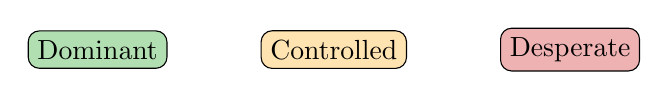
\begin{tikzpicture}
  \node[draw,rounded corners,fill=dominant!30] (d) at (0,0) {Dominant};
  \node[draw,rounded corners,fill=controlled!30] (c) at (3,0) {Controlled};
  \node[draw,rounded corners,fill=desperate!30] (e) at (6,0) {Desperate};
\end{tikzpicture}
&
\textbf{Effect:} &

\begin{tikzpicture}
  \node[draw,rounded corners,fill=green!30] (l) at (0,0) {Limited};
  \node[draw,rounded corners,fill=blue!30] (s) at (3,0) {Standard};
  \node[draw,rounded corners,fill=orange!30] (g) at (6,0) {Great};
\end{tikzpicture}
\end{tabularx}
\vspace{0.3cm}

% -----------------------------------------------------------------
% 4. Boons & Story Beats (SB)
% -----------------------------------------------------------------
\noindent\begin{tabularx}{\linewidth}{@{}L{3.2cm} C{4cm} C{4cm}@{}}
\textbf{Boons (max 5):} &

\begin{tikzpicture}
  \foreach \i in {1,...,5}{
    \draw (\i*1.2,0) circle (0.4);
  }
\end{tikzpicture}
&
\textbf{Story Beats (SB) Bank (max 12):}\\
\smallskip
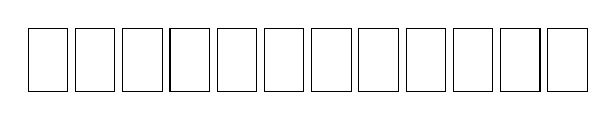
\begin{tikzpicture}
  \foreach \i in {1,...,12}{
    \draw (\i*0.6,0) rectangle (0.5+\i*0.6,0.8);
  }
\end{tikzpicture}
\end{tabularx}
\vspace{0.5cm}

% -----------------------------------------------------------------
% 5. Skills (two‑column table)
% -----------------------------------------------------------------
\section*{Skills (rating 0‑5)}
\noindent\begin{tabularx}{\linewidth}{@{} L{4.5cm} C{1.2cm} C{1.2cm} L{4.5cm} C{1.2cm} C{1.2cm} @{}}
\textbf{Melee}        & \underline{\hspace{1cm}} &  & \textbf{Stealth}     & \underline{\hspace{1cm}} &   \\
\textbf{Ranged}       & \underline{\hspace{1cm}} &  & \textbf{Subterfuge} & \underline{\hspace{1cm}} &   \\
\textbf{Athletics}    & \underline{\hspace{1cm}} &  & \textbf{Sway}       & \underline{\hspace{1cm}} &   \\
\textbf{Brawl}        & \underline{\hspace{1cm}} &  & \textbf{Diplomacy}  & \underline{\hspace{1cm}} &   \\
\textbf{Command}      & \underline{\hspace{1cm}} &  & \textbf{Investigate}& \underline{\hspace{1cm}} &   \\
\textbf{Craft (Tinker)}& \underline{\hspace{1cm}} &  & \textbf{Lore}       & \underline{\hspace{1cm}} &   \\
\textbf{Arcana}       & \underline{\hspace{1cm}} &  & \textbf{Notice}     & \underline{\hspace{1cm}} &   \\
\textbf{Medicine}      & \underline{\hspace{1cm}} &  & \textbf{Performance}& \underline{\hspace{1cm}} &   \\
\textbf{Survival}     & \underline{\hspace{1cm}} &  & \textbf{Presence}   & \underline{\hspace{1cm}} &   \\
\textbf{Endurance}    & \underline{\hspace{1cm}} &  &                     &                           &   \\
\end{tabularx}
\vspace{0.5cm}

% -----------------------------------------------------------------
% 6. Talents (list with cost)
% -----------------------------------------------------------------
\section*{Talents}
\begin{tabularx}{\linewidth}{@{} L{7cm} C{2cm} X @{}}
\cmark\ \textbf{Spellcraft} (6 XP) & 6 XP & Freeform elemental casting – Weave + Cast.\\
\cmark\ \textbf{Familiar} (2 XP)   & 2 XP & Provides Patron’s Gift and minor imbuements.\\
\blankbox\ \textbf{Weapon Master} (5 XP) & 5 XP & +2 dice with chosen weapon class.\\
\blankbox\ \textbf{Tactical Movement} (4 XP) & 4 XP & Move as an Action while engaged.\\
\blankbox\ \textbf{Defensive Survival} (3 XP) & 3 XP & +1 die to defence rolls, once/scene convert Harm 1 → Fatigue.\\
% add more rows as needed
\end{tabularx}
\vspace{0.5cm}

% -----------------------------------------------------------------
% 7. Assets & Followers (quick‑reference)
% -----------------------------------------------------------------
\section*{Assets \& Followers}
\noindent\begin{tabularx}{\linewidth}{@{} L{4.5cm} C{2.5cm} L{6cm} @{}}
\textbf{Asset} & \textbf{Status} & \textbf{Boon Cost / Effect}\\
Family Heirloom Dagger & Maintained & 1 Bo​n – +1 die (Melee) for this scene.\\
Patron’s Symbol (Ikasha) & Maintained & 1 Bo​n – +1 die to Stealth‑type spells.\\
\midrule
\textbf{Follower} & \textbf{Role / Assist} & \textbf{Notes}\\
Joran – Scout & +1 die (Assist) & Grants +1 die to any nearby roll.\\
Mira – Quartermaster & +1 die (Assist) & Provides +1 die to any Supply‑type check.\\
\end{tabularx}
\vfill
\newpage

% =============================================================
% ========================  BACK PAGE  =======================
% =============================================================

\section*{Back – Detailed Bookkeeping}

% -------------------------------------------------------------
%  A. Health – Harm / Fatigue (repeat for quick reference)
% -------------------------------------------------------------
\noindent\begin{tabularx}{\linewidth}{@{} L{3.2cm} C{4cm} C{4cm} C{4cm}@{}}
\textbf{Harm Tracker} &
\begin{tikzpicture}
  \foreach \i/\col in {1/red,2/orange,3/black}{
    \draw[fill=\col!30] (0,-\i) rectangle (0.8,-\i-0.8);
  }
  \node[left] at (-0.2,-1.5) {Level 1};
  \node[left] at (-0.2,-2.5) {Level 2};
  \node[left] at (-0.2,-3.5) {Level 3};
\end{tikzpicture}
&
\textbf{Fatigue Tracker (Body)} &
\begin{tikzpicture}
  \foreach \i in {1,...,5}{
    \draw (0,-\i) rectangle (0.8,-\i-0.8);
  }
  \node[left] at (-0.2,-3.5) {Add a mark for each point of fatigue.};
\end{tikzpicture}
\end{tabularx}
\vspace{0.6cm}

% -------------------------------------------------------------
%  B. Obligation & Corruption clocks
% -------------------------------------------------------------
\section*{Obligation / Corruption}
\noindent\begin{tabularx}{\linewidth}{@{} L{4.5cm} C{6cm} @{}}
\textbf{Patron Obligation (per Patron)} &
\begin{tikzpicture}
  \foreach \i in {1,...,6}{
    \draw (0,-\i) rectangle (1.4,-\i-0.8);
  }
  \node[left] at (-0.2,-2) {Mark a segment each time you invoke a Rite.};
\end{tikzpicture}\\[0.2cm]
\textbf{Corruption Clock (if applicable)} &
\begin{tikzpicture}
  \foreach \i in {1,...,5}{
    \draw (0,-\i) rectangle (1.4,-\i-0.8);
  }
  \node[left] at (-0.2,-2) {Mark when you Push a spell, take heavy backlash, etc.};
\end{tikzpicture}
\end{tabularx}
\vspace{0.6cm}

% -------------------------------------------------------------
%  C. Active Clocks (Scene / Journey / Campaign)
% -------------------------------------------------------------
\section*{Active Clocks}
\noindent\begin{tabularx}{\linewidth}{@{} L{3.5cm} C{5cm} L{3.5cm} C{5cm} @{}}
\textbf{Scene Clock} &
\begin{tikzpicture}
  \foreach \i in {1,...,6}{
    \draw (0,-\i) rectangle (1.4,-\i-0.8);
  }
  \node[left] at (-0.2,-2) {e.g. “Guards Alerted”.};
\end{tikzpicture}
&
\textbf{Journey Clock} &
\begin{tikzpicture}
  \foreach \i in {1,...,6}{
    \draw (0,-\i) rectangle (1.4,-\i-0.8);
  }
  \node[left] at (-0.2,-2) {e.g. “Crossing the Mist”.};
\end{tikzpicture}\\[0.2cm]
\textbf{Campaign Clock} &
\begin{tikzpicture}
  \foreach \i in {1,...,8}{
    \draw (0,-\i) rectangle (1.8,-\i-0.8);
  }
  \node[left] at (-0.2,-3) {e.g. “Patron’s Favor”.};
\end{tikzpicture}
&
 &
\end{tabularx}
\vspace{0.6cm}

% -------------------------------------------------------------
%  D. Magic – TAGS & Freeform Casting
% -------------------------------------------------------------
\section*{Magic – Freeform Casting (Caster Path)}
\noindent\begin{tabularx}{\linewidth}{@{} L{4cm} C{10cm} @{}}
\textbf{Spell Intent} &
\underline{\hspace{12cm}} % player writes a short description
\\[0.3cm]
\textbf{Tags (check all that apply)} &
\begin{tabular}{l l l l}
[AREA]   & [WARD]   & [BURNING] & [FORCE] \\
[HEAL]   & [DISPEL] & [VEIL]    & [REVEAL] \\
[SUMMON] & [TRAP]   & [BOUND]   & [CHARGE] \\
\end{tabular}
\\[0.3cm]
\textbf{DV} & 1 + (number of tags)  (dangerous tags add +2)\\
\textbf{Position} & (Dominant / Controlled / Desperate)\\
\textbf{Effect}   & (Limited / Standard / Great)\\
\end{tabularx}
\vspace{0.4cm}

% -------------------------------------------------------------
%  E. Rites / Symbols – Runekeeper & Invoker
% -------------------------------------------------------------
\section*{Rites (Runekeeper) / Symbols (Invoker)}
\noindent\begin{tabularx}{\linewidth}{@{} L{3.5cm} C{12cm} @{}}
\textbf{Rite Name} &
\underline{\hspace{10cm}}
\\[0.2cm]
\textbf{Patron} & \underline{\hspace{6cm}}\\
\textbf{Obligation Cost} & \underline{\hspace{3cm}} \\
\textbf{DV (base)} & \underline{\hspace{3cm}} \\
\textbf{Push?} & \checkbox\ \ (adds +1 Obligation)\\
\textbf{Effect / Tags} &
\underline{\hspace{10cm}}
\\[0.2cm]\midrule
% duplicate the block as many times as you like
\textbf{Rite Name} &
\underline{\hspace{10cm}}
\\[0.2cm]
\textbf{Patron} & \underline{\hspace{6cm}}\\
\textbf{Obligation Cost} & \underline{\hspace{3cm}} \\
\textbf{DV (base)} & \underline{\hspace{3cm}} \\
\textbf{Push?} & \checkbox\ \ (adds +1 Obligation)\\
\textbf{Effect / Tags} &
\underline{\hspace{10cm}}
\\
\end{tabularx}
\vspace{0.4cm}

% -------------------------------------------------------------
%  F. Equipment – Weapons, Armor, Gear, Enchantments
% -------------------------------------------------------------
\section*{Equipment}
\noindent\begin{tabularx}{\linewidth}{@{} L{4cm} C{2cm} C{2cm} C{2cm} C{4cm} @{}}
\textbf{Item} & \textbf{Weight} & \textbf{Dice} & \textbf{Tags} & \textbf{Condition}\\
Longsword (Medium) & Medium & +1 d & \blankbox\ \textit{Reach} & Maintained\\
Leather Armor (Light) & Light & –1 d (to attacks) & \blankbox\ \textit{Stealth} & Compromised\\
Heirloom Dagger & Light & +1 d (Melee) & \blankbox\ \textit{Quickdraw} & Maintained\\
Lock‑pick Set (Tinker) & Light & – & – & Maintained\\
\end{tabularx}
\vspace{0.4cm}

% -------------------------------------------------------------
%  G. Notes, Bonds, Complications, Quick‑Refs
% -------------------------------------------------------------
\section*{Notes / Bonds / Complications}
\begin{minipage}[t]{0.48\linewidth}
\textbf{Bonds (max 3)}\\[0.2cm]
\begin{enumerate}[leftmargin=*]
  \item \underline{\hspace{8cm}}
  \item \underline{\hspace{8cm}}
  \item \underline{\hspace{8cm}}
\end{enumerate}
\end{minipage}
\hfill
\begin{minipage}[t]{0.48\linewidth}
\textbf{Complications}\\[0.2cm]
\begin{itemize}[leftmargin=*]
  \item \underline{\hspace{8cm}}
  \item \underline{\hspace{8cm}}
  \item \underline{\hspace{8cm}}
\end{itemize}
\end{minipage}

\vspace{0.4cm}
\textbf{Quick Reference (cheat‑sheet)}\\
\begin{tabular}{ll}
Assist (→ +1 die)                     & \cmark\ \textit{once/scene}\\
Shift Position (pay 1 Bo​n)           & \cmark\ \textit{Dominant ↔ Controlled ↔ Desperate}\\
Re‑roll a die (spend 1 Bo​n)         & \cmark\\
Activate Asset (spend 1 Bo​n)         & \cmark\\
Push a spell (add Obligation)        & \cmark\\
\end{tabular}

\end{document}

